% You should title the file with a .tex extension (hw1.tex, for example)
\documentclass[12pt]{article}\sloppy

\usepackage{amsmath,bm}
\usepackage{amssymb}
\usepackage{fancyhdr}
\usepackage{graphicx}
\usepackage{float}
\usepackage{longtable}

\floatplacement{figure}{H}
\oddsidemargin0cm
\topmargin-2cm     %I recommend adding these three lines to increase the 
\textwidth16.5cm   %amount of usable space on the page (and save trees)
\textheight23.5cm  

\newcommand{\myname}{Abhinav Maurya}
\newcommand{\myandrew}{amaurya@andrew.cmu.edu}
\newcommand{\myhwnum}{3}

\newcommand{\question}[2] {\vspace{.25in} \hrule\vspace{0.5em} \noindent{\bf #1: #2} \vspace{0.5em} \hrule \vspace{.10in}}
\renewcommand{\part}[1] {\vspace{.10in} {\bf (#1)}}

\setlength{\parindent}{0pt}
\setlength{\parskip}{5pt plus 1pt}
 
\pagestyle{fancyplain}
\lhead{\fancyplain{}{\textbf{HW\myhwnum}}}      % Note the different brackets!
\rhead{\fancyplain{}{\myname\\ \myandrew}}
\chead{\fancyplain{}{16-720}}

\begin{document}

\medskip                        % Skip a "medium" amount of space
                                % (latex determines what medium is)
                                % Also try: \bigskip, \littleskip

\thispagestyle{plain}
\begin{center}                  % Center the following lines
{\Large 16-720: Assignment \myhwnum} \\
\myname \\
\myandrew \\
\end{center}

\question{1.1.1}{Nature of $A'A$}

When we linearize the optimization objective for Lucas-Kanade alignment (given below), we get loading matrix $A$ which has two columns, one for gradients along X-direction and the second for gradients along Y-direction. Therefore, $A'A$ is a 2x2 Hessian matrix which is computed using the gradients of the image. The $A' \Delta u = b$ linearized equation is as follows: $$[Dx,Dy]*[\Delta u, \Delta v]' = \Delta I$$ Here $\Delta I$ is the difference between consecutive template windows, where the successor template window is at a displacement of $u,v$ with respect to the previous tracking window. Intuitively, we are trying to perform a first-order approximation by equating the change in successive template windows with the product of gradients (rate of change) and the $u,v$ column vector (actual displacement). The optimization is performed iteratively starting with $u,v=0$.

$$[Dx,Dy]*[\Delta u, \Delta v]' = \Delta I_t$$

$$A \Delta p = \Delta I$$

$$A' A \Delta p = A' \Delta I$$

$$\Delta p = (A' A) \backslash (A' \Delta I)$$

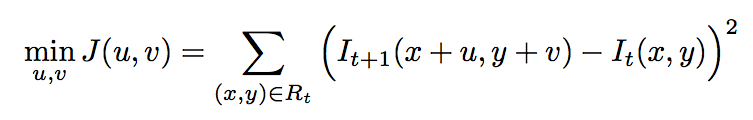
\includegraphics[width=0.8\linewidth]{eq1.png}

\question{1.1.2}{Conditions on $A'A$}

$A'A$ needs to be well-conditioned so that it is invertible. It implies that none of its eigenvalues can be zero or very close to zero. Eigenvalues of the inverted resulting matrix are reciprocals of the eigenvalues of the matrix being inverted. If any eigenvalue is zero or close to zero, inverting the matrix will lead to infinite or very high eigenvalues of the inverted matrix which can lead to problems in finite-precision calculations. The ratio of the largest eigenvalue to smallest eigenvalue called the conditioning number of a matrix cannot be very small.

\question{1.2}{LucasKanade}

Included in \texttt{code/LucasKanade.m} file.

\question{1.3}{testCarSequence}

Included in \texttt{code/testCarSequence.m} file. Results in figure (\ref{fig:testcarsequence})

\begin{figure*}[f]
\centering
\begin{tabular}{c c c c c}
  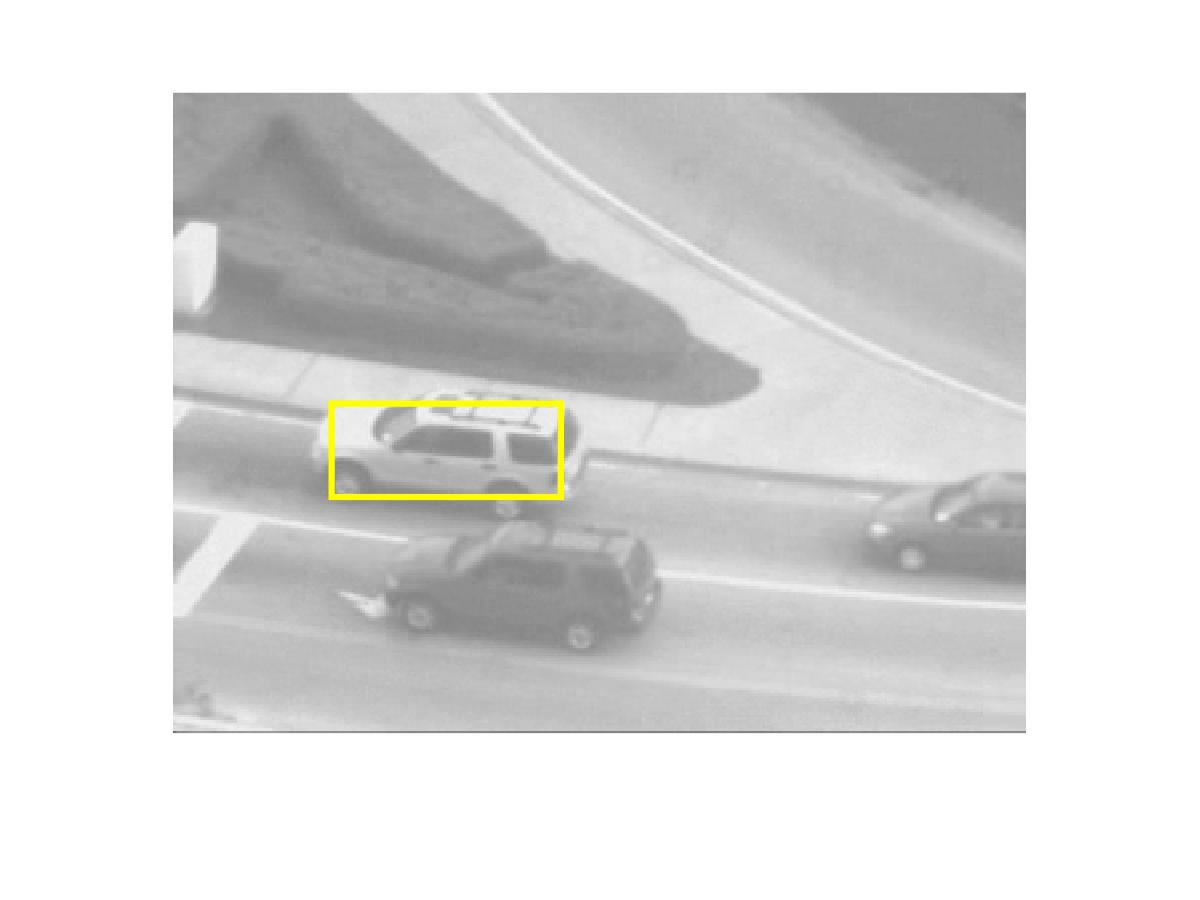
\includegraphics[trim=60mm 60mm 60mm 60mm,clip=true,width=0.18\linewidth]{../results/CarFrame1.jpg} & 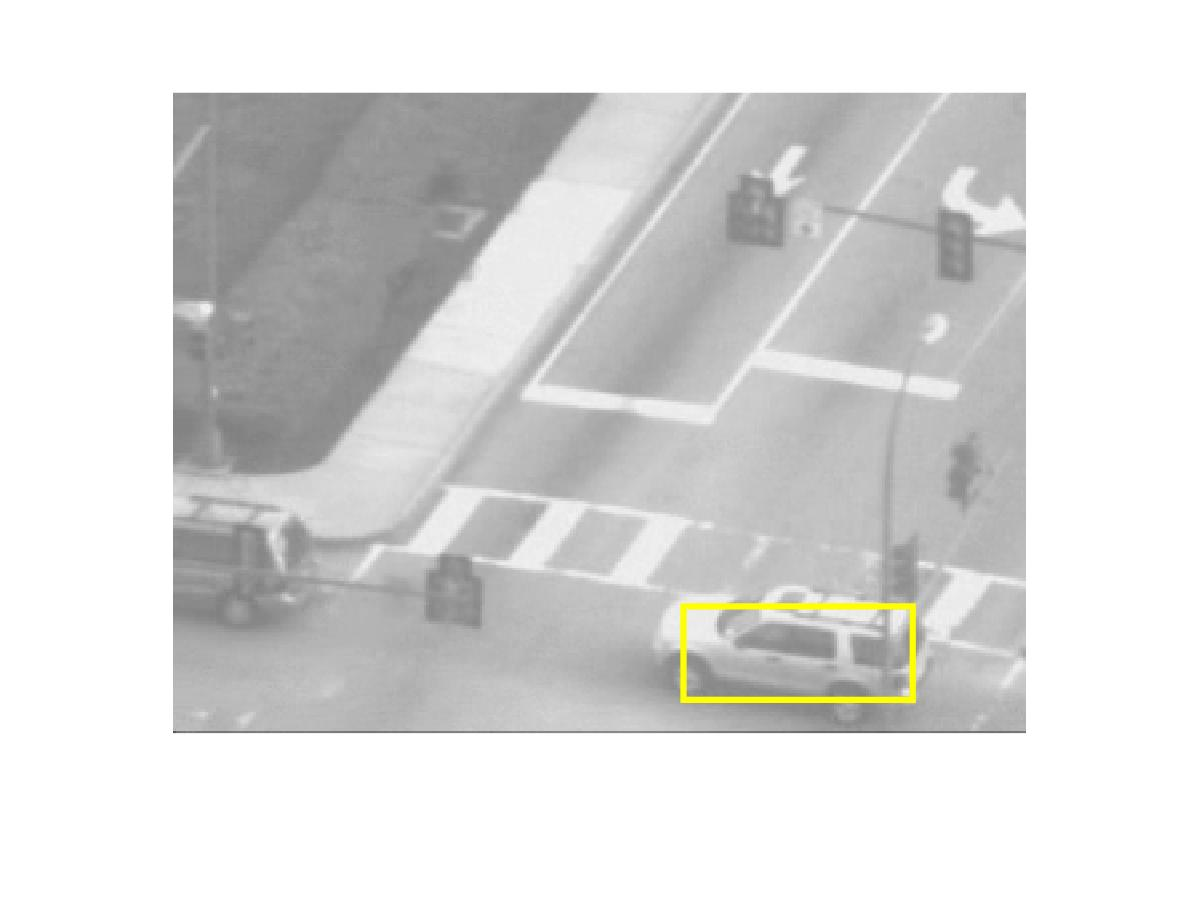
\includegraphics[trim=60mm 60mm 60mm 60mm,clip=true,width=0.18\linewidth]{../results/CarFrame100.jpg} & 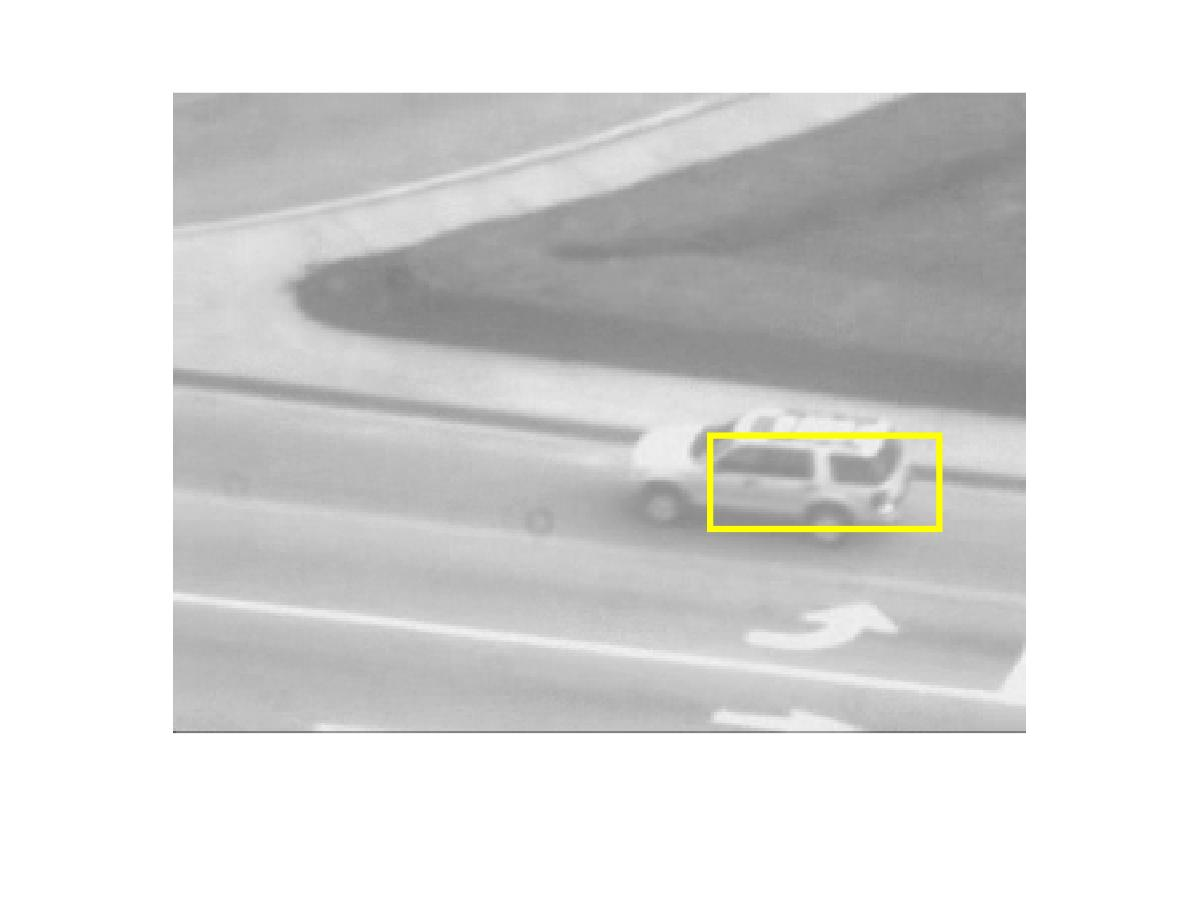
\includegraphics[trim=60mm 60mm 60mm 60mm,clip=true,width=0.18\linewidth]{../results/CarFrame200.jpg} & 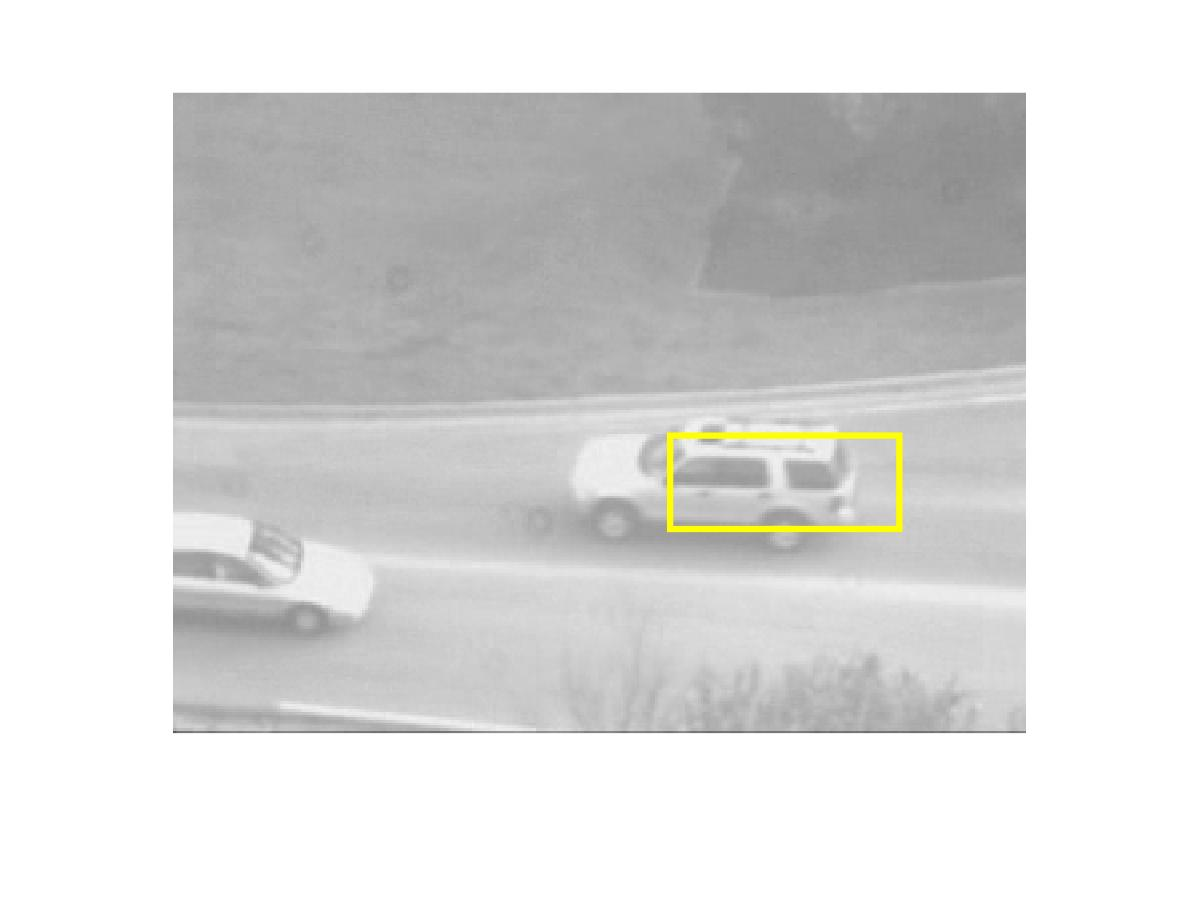
\includegraphics[trim=60mm 60mm 60mm 60mm,clip=true,width=0.18\linewidth]{../results/CarFrame300.jpg} & 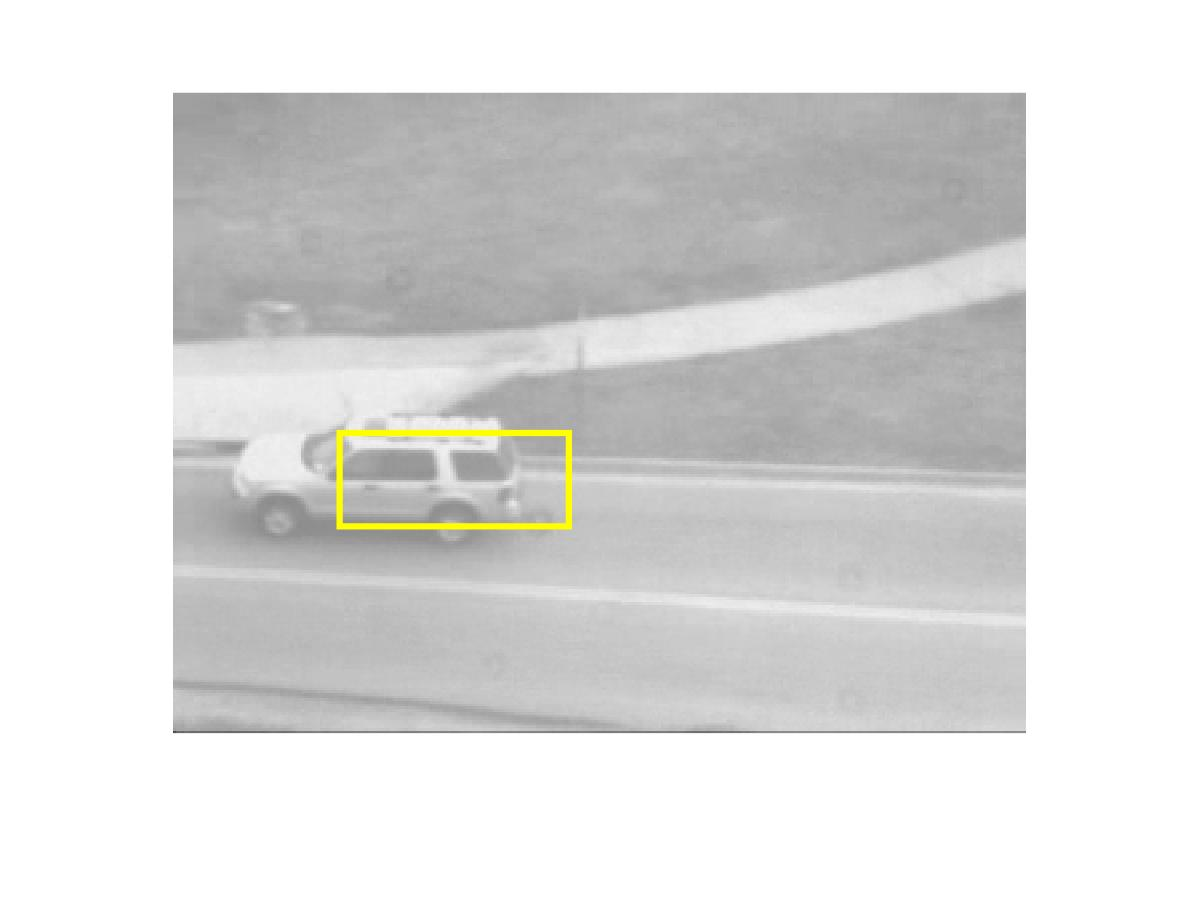
\includegraphics[trim=60mm 60mm 60mm 60mm,clip=true,width=0.18\linewidth]{../results/CarFrame400.jpg} \\
\end{tabular}
\caption{Output of \texttt{testCarSequence}}
\label{fig:testcarsequence}
\end{figure*}

\question{1.4}{testCarSequenceWithTemplateCorrection}

Included in \texttt{code/testCarSequenceWithTemplateCorrection.m} file. Results in figure (\ref{fig:testcarsequencewithtemplatecorrection})

We used the \texttt{code/subtractDominantMotion.m} function written as part of this assignment to improve the tracking. Every 50 frames, we computed the mask using the \texttt{code/subtractDominantMotion.m} function, performed a search over altertive rectangles around the current rectangle (+/-5 pixels both horizontally and vertically), and chose an alternate rectangle if it improved a score by at least a certain positove amount (100 in our case). The score of competing rectangles was calculated using the mask image by counting the number of pixels in the mask image corresponding to the rectangle which were detected to contain a fast moving object against a slower moving background. The results were visibly better and the slight optimization allowed the tracked rectangle to refocus on the object. Since the top and windows of the car have the maximum contrast, the tracking rectangle latches onto this aspect and tracks it throughout the video. 

\begin{figure*}[f]
\centering
\begin{tabular}{c c c c c}
  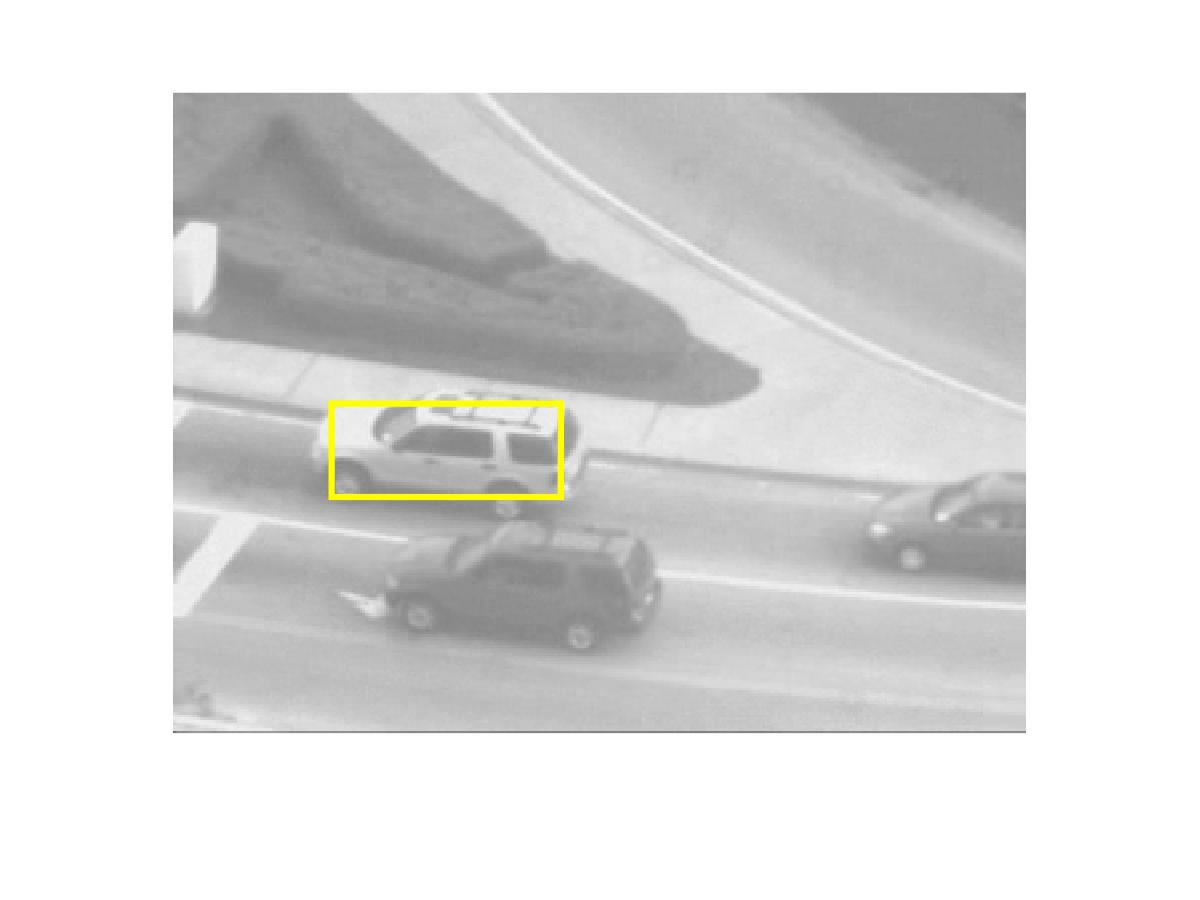
\includegraphics[trim=60mm 60mm 60mm 60mm,clip=true,width=0.18\linewidth]{../results/yCarFrame1.jpg} & 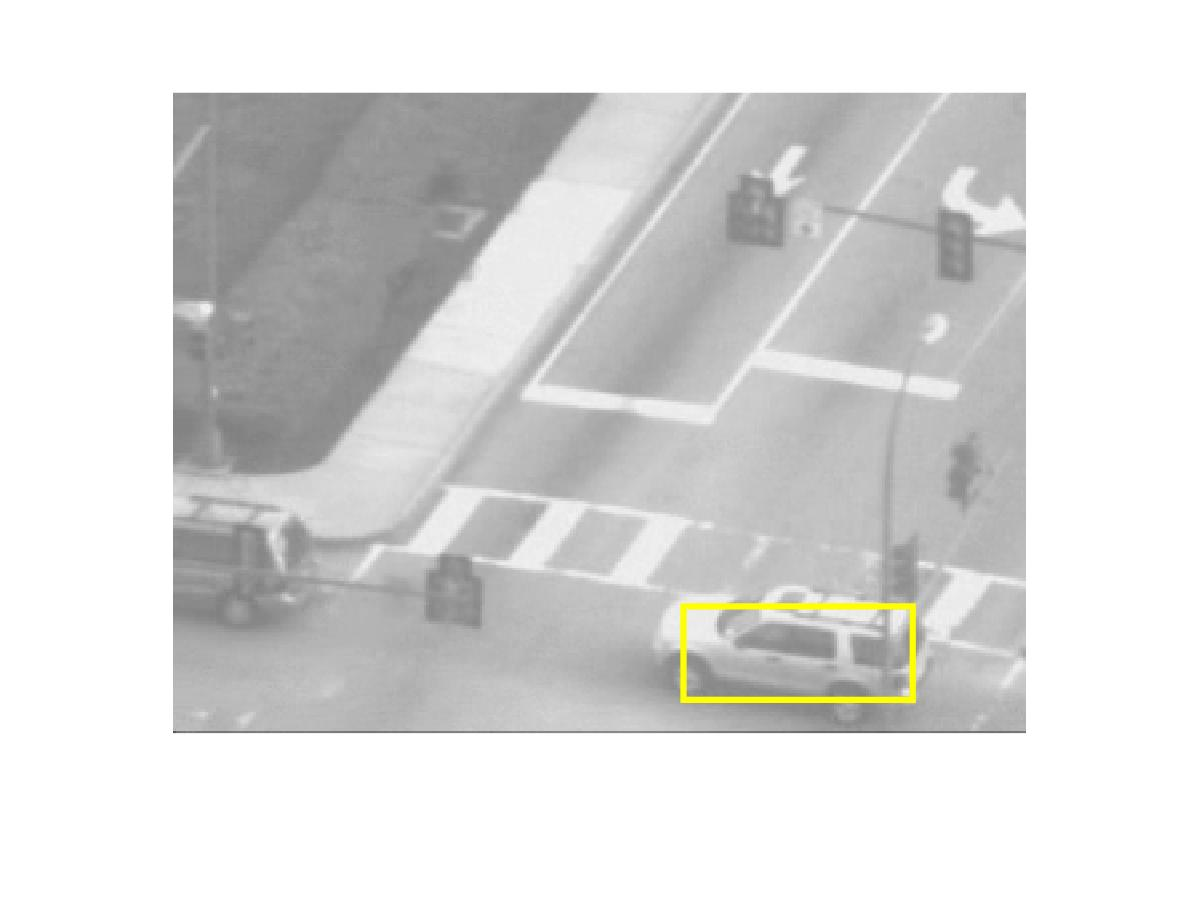
\includegraphics[trim=60mm 60mm 60mm 60mm,clip=true,width=0.18\linewidth]{../results/yCarFrame100.jpg} & 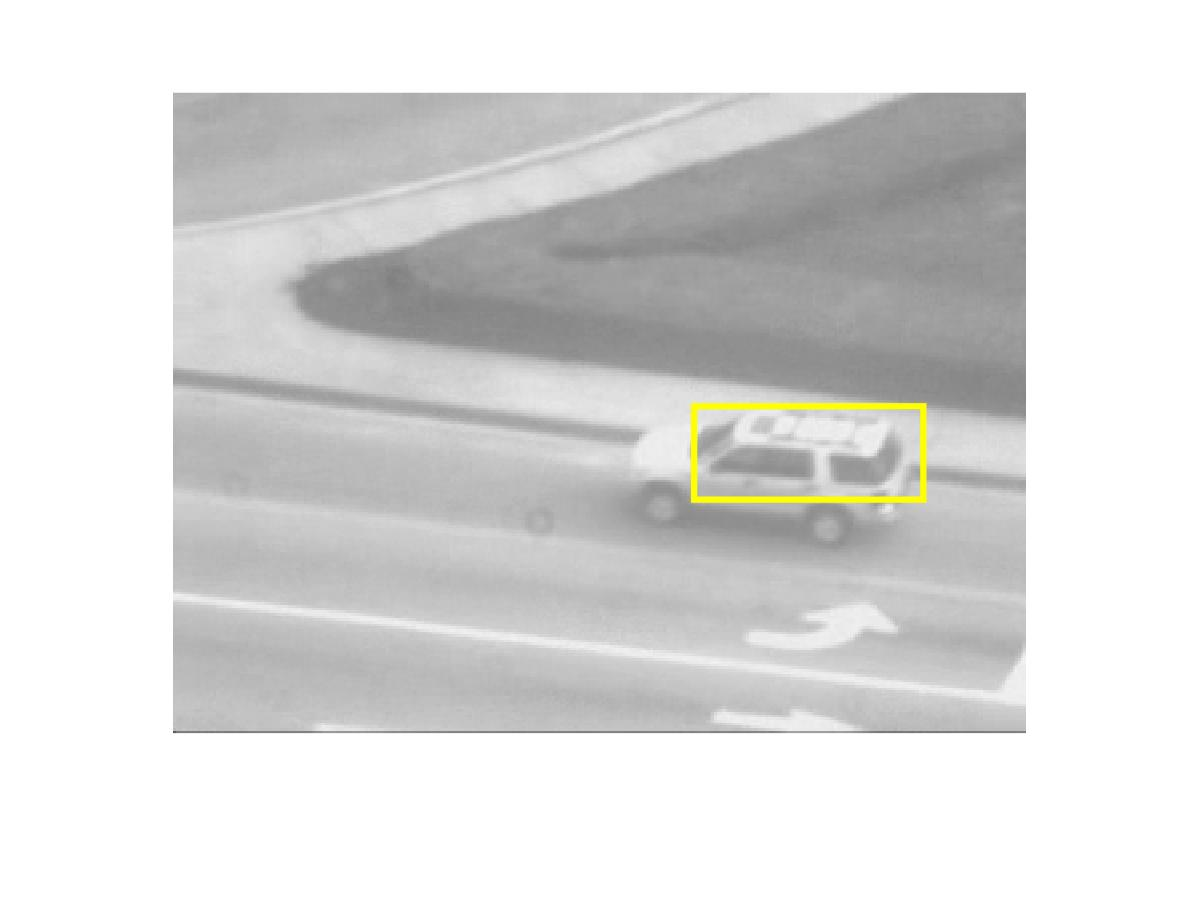
\includegraphics[trim=60mm 60mm 60mm 60mm,clip=true,width=0.18\linewidth]{../results/yCarFrame200.jpg} & 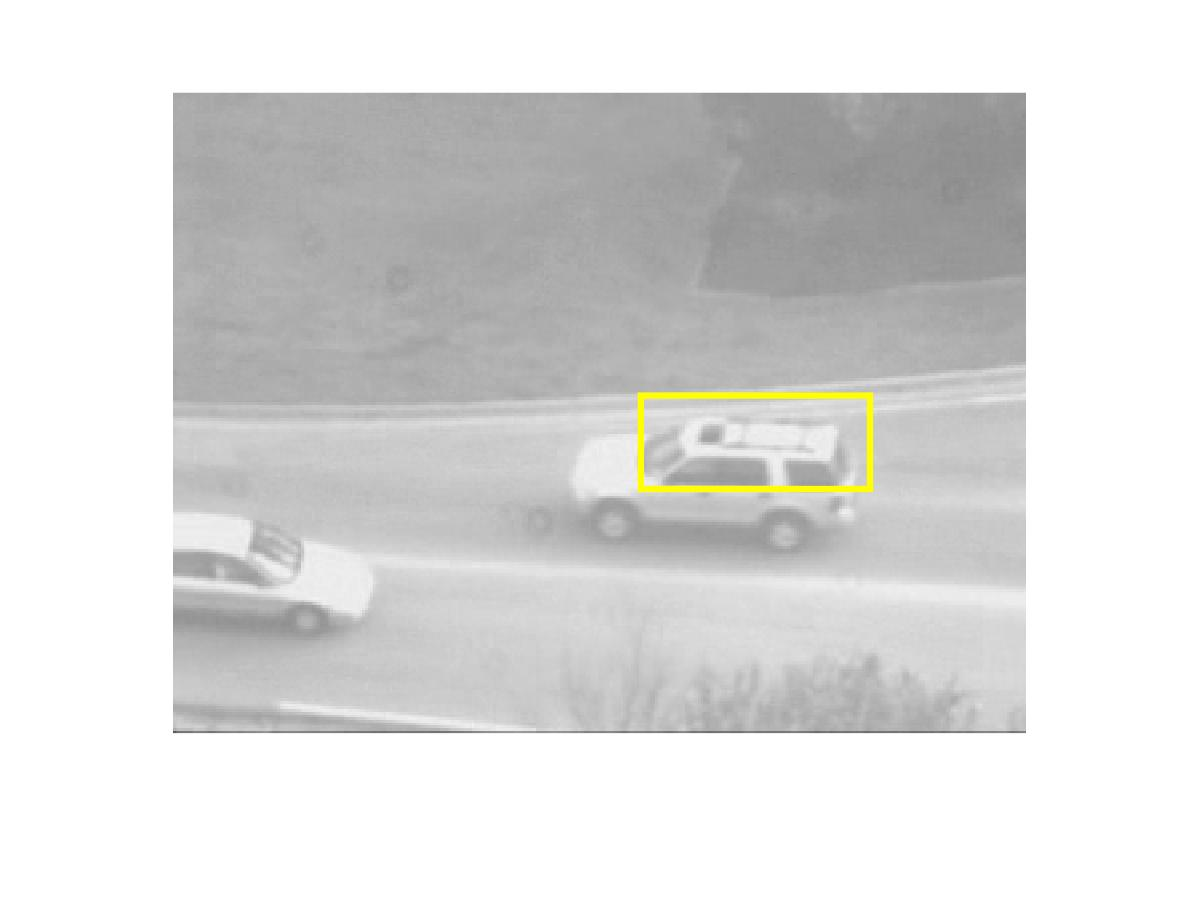
\includegraphics[trim=60mm 60mm 60mm 60mm,clip=true,width=0.18\linewidth]{../results/yCarFrame300.jpg} & 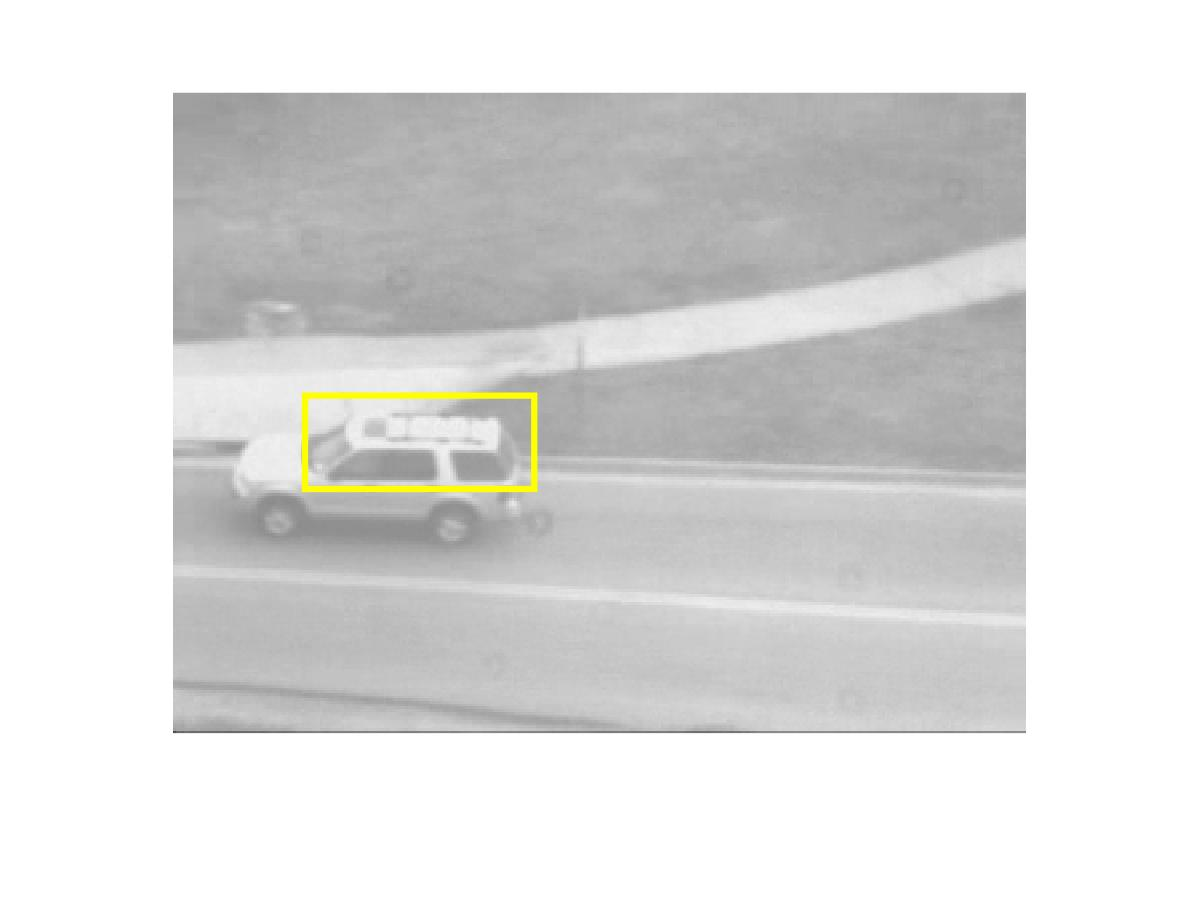
\includegraphics[trim=60mm 60mm 60mm 60mm,clip=true,width=0.18\linewidth]{../results/yCarFrame400.jpg} \\
\end{tabular}
\caption{Output of \texttt{testCarSequenceWithTemplateCorrection}}
\label{fig:testcarsequencewithtemplatecorrection}
\end{figure*}

\question{2.1}{Weight vector for basis functions}

We are given that $$\sum_{c=1..C} w_c B_c = I_{t+1}-I_t$$

Since the basic images $B_i$ are othogonal to each other, we multiply both sides by $B_c'$ if we are trying to determine $w_c$.

$$w_c B_c' B_c + \sum_{i=1..C:i \neq c} w_i B_c' B_i = B_c' (I_{t+1}-I_t)$$

$$\therefore w_c B_c' B_c = B_c' (I_{t+1}-I_t)$$

$$\therefore w_c = (B_c' B_c) \backslash (B_c' (I_{t+1}-I_t))$$

The weight vector $w_c$ is essentially discovered as a solution to the optimization problem mentioned in the assignment. 

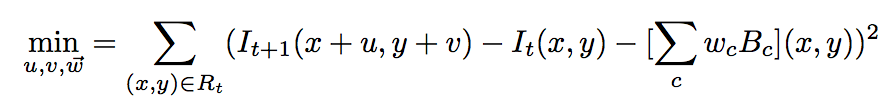
\includegraphics[width=0.8\linewidth]{eq2.png}

As we see, it is an extension to the original Lucas-Kanade optimization problem we optimized for in question (1). We naturally extend the original Lucas-Kanade optimization procedure by extending the optimization vector from $[u,v]$ to $[u,v,\bm{w_c}]$. The basis vectors are linearized into column vectors are appended to the original $A=[Dx,Dy]$ matrix. Thus, $A=[Dx,Dy,B_1,B_2,...,B_n]$ where $B_1,B_2,...,B_n$ are the $n$ provided basis functions that can explain the shifted template in the succesor image in addition to the gradients from the predecessor image. Thus, the linearization is transformed as follows:

$$[Dx,Dy,B_1,B2,...,B_n]*[\Delta u, \Delta v, w_1, w_2, ..., w_n]' = \Delta I_t$$

$$A \Delta p = \Delta I$$

$$A' A \Delta p = A' \Delta I$$

$$\Delta p = (A' A) \backslash (A' \Delta I)$$

While $\Delta u, \Delta v$ are optimized cumulatively, weights $w_c$ are solved afresh every time we incrementally search for a new $\Delta u, \Delta v$. This is because the basis vectors are constants and are not changing with the optimization like $Dx,Dy$.

\question{2.2}{LucasKanadeBasis}

Included in \texttt{code/LucasKanadeBasis.m} file.

\question{2.3}{testSylvSequence}

Included in \texttt{code/testSylvSequence.m} file. Results in figure (\ref{fig:testsylvsequence}).

\begin{figure*}[f]
\centering
\begin{tabular}{c c c c c}
  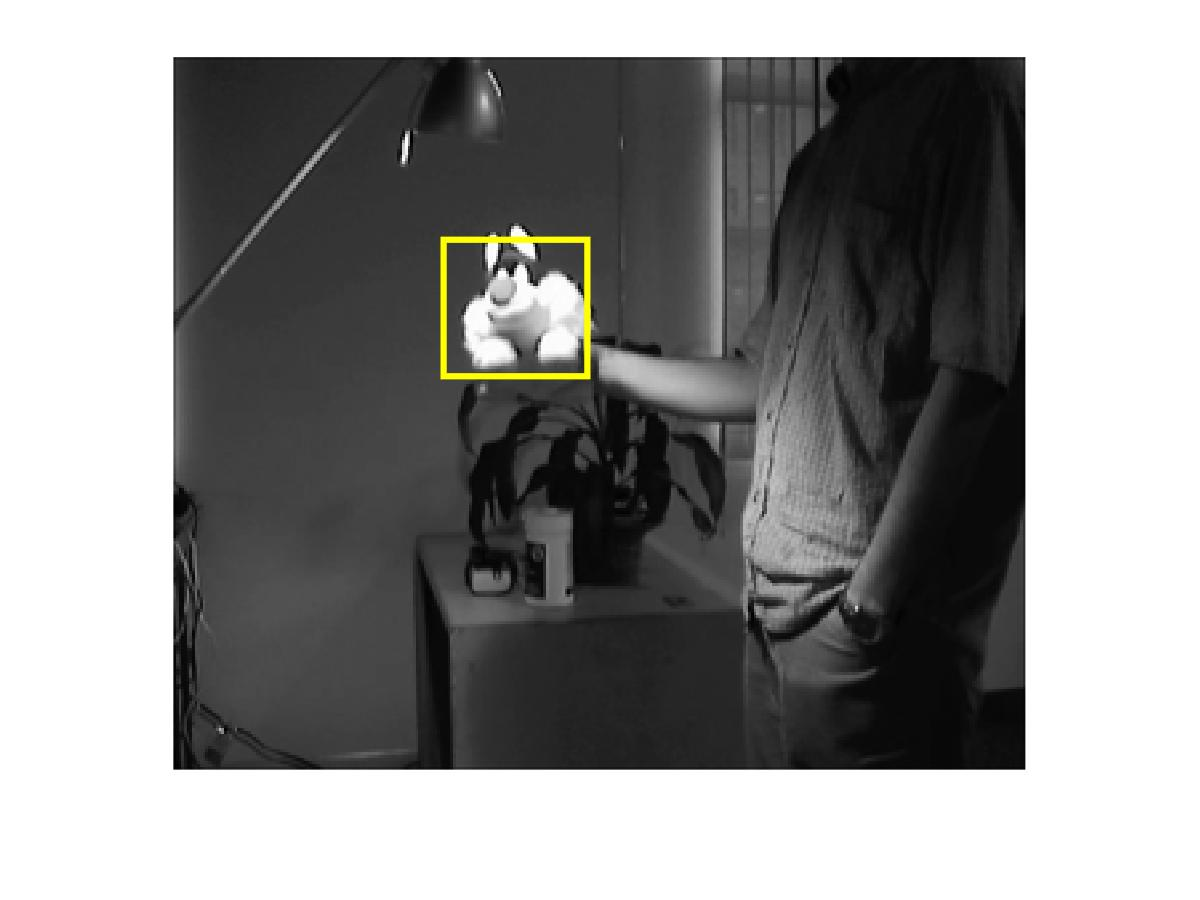
\includegraphics[trim=60mm 60mm 60mm 60mm,clip=true,width=0.18\linewidth]{../results/SylvFrame1.jpg} & 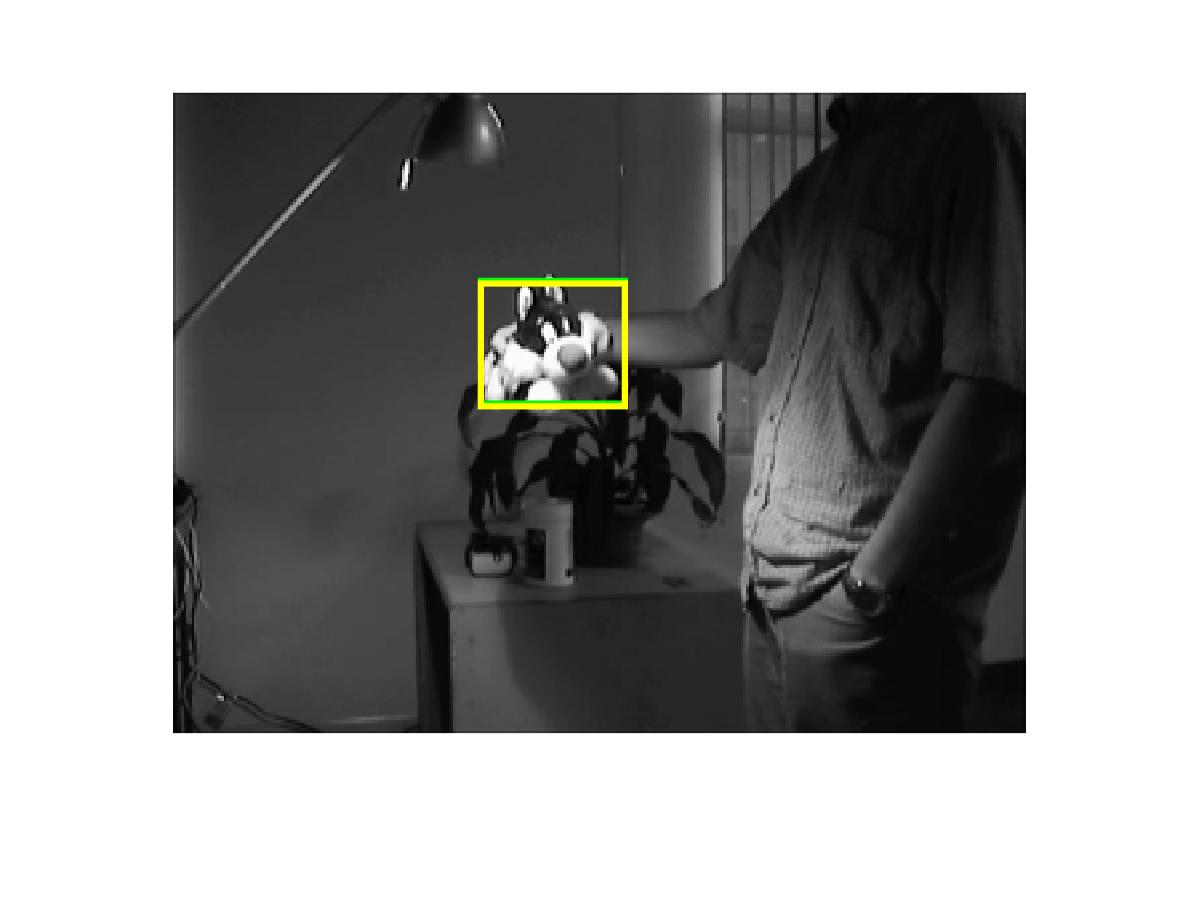
\includegraphics[trim=60mm 60mm 60mm 60mm,clip=true,width=0.18\linewidth]{../results/SylvFrame200.jpg} & 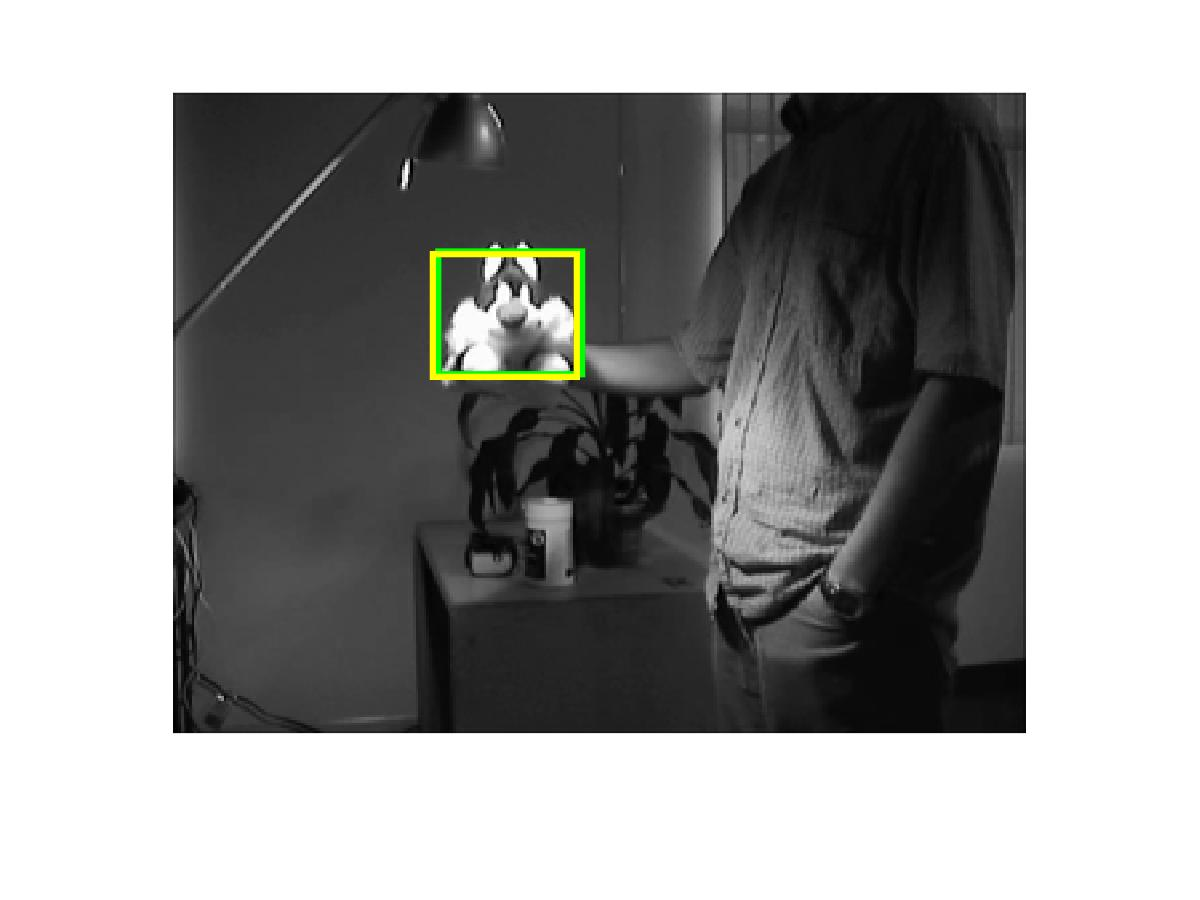
\includegraphics[trim=60mm 60mm 60mm 60mm,clip=true,width=0.18\linewidth]{../results/SylvFrame300.jpg} & 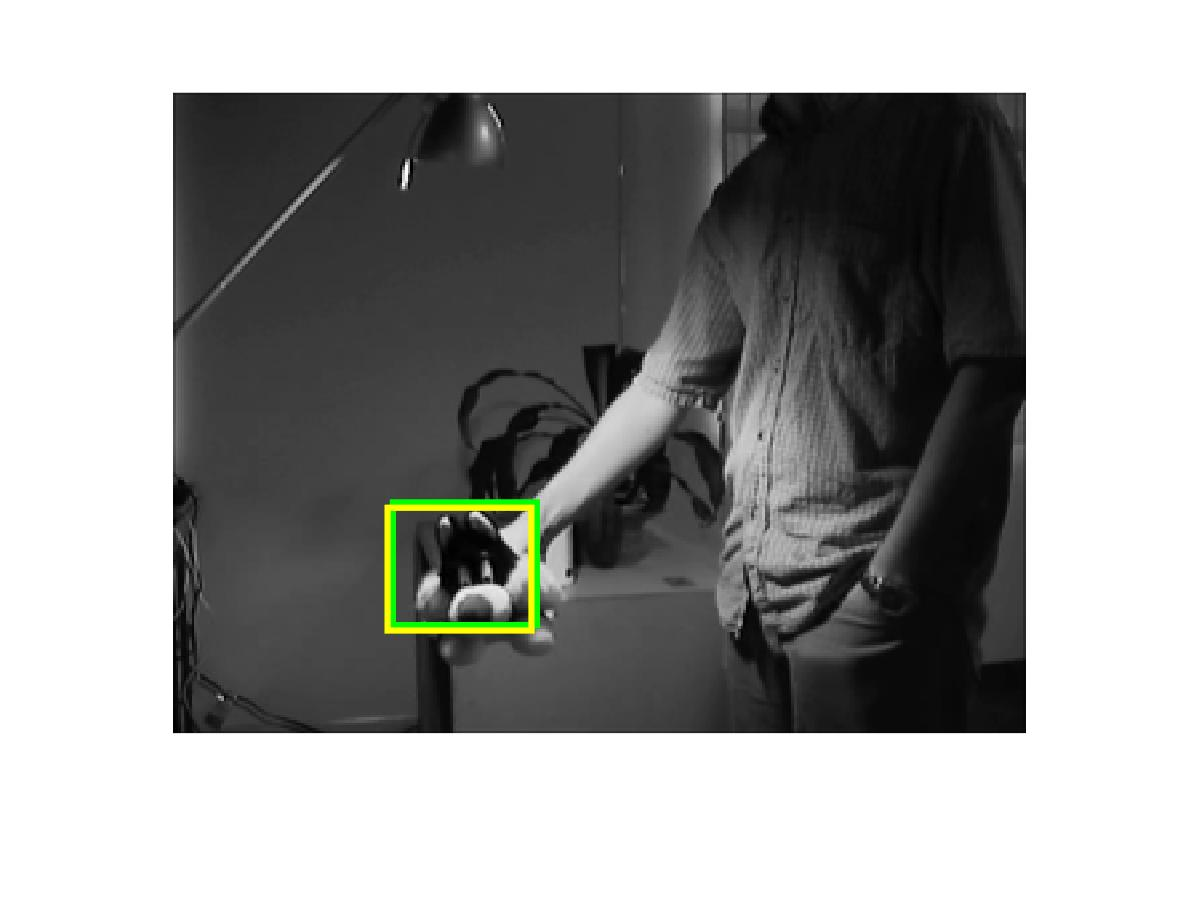
\includegraphics[trim=60mm 60mm 60mm 60mm,clip=true,width=0.18\linewidth]{../results/SylvFrame350.jpg} & 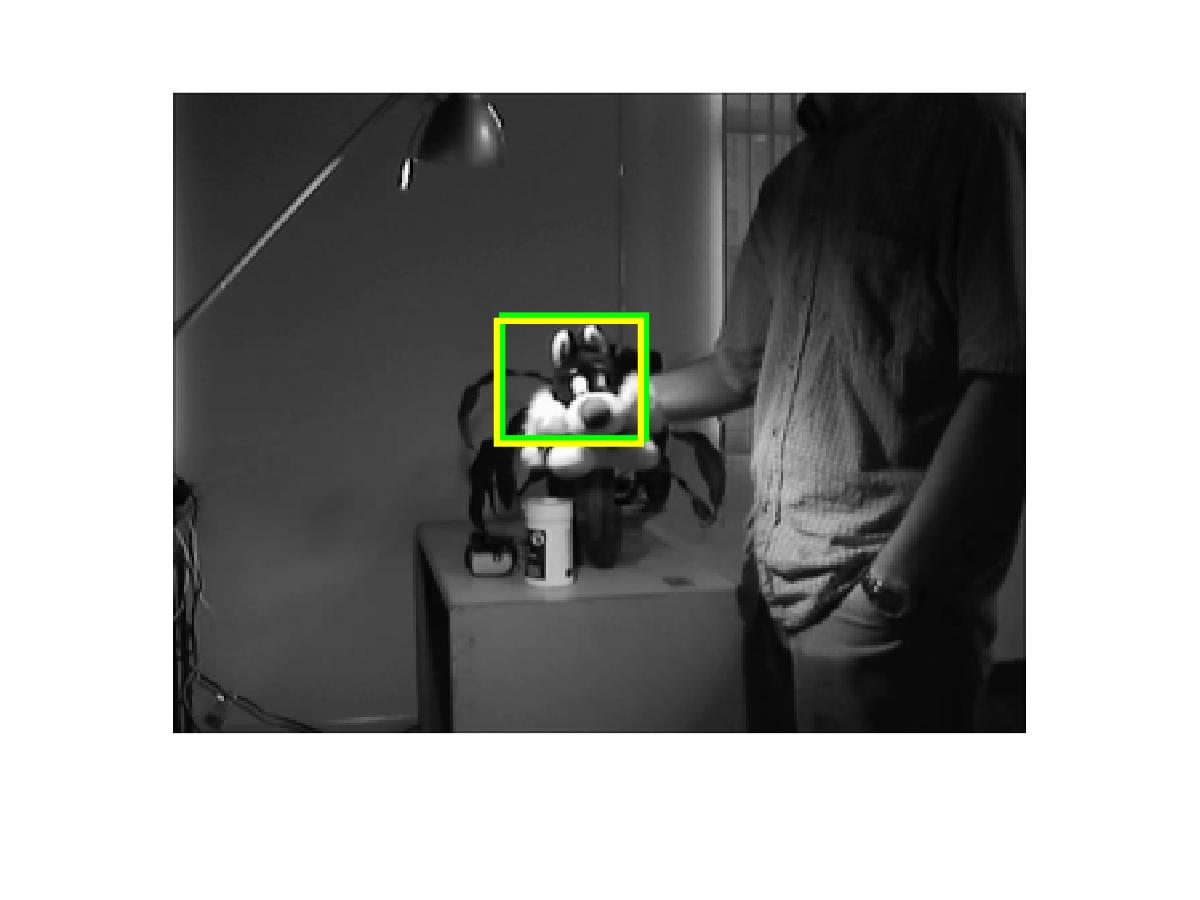
\includegraphics[trim=60mm 60mm 60mm 60mm,clip=true,width=0.18\linewidth]{../results/SylvFrame400.jpg} \\
\end{tabular}
\caption{Output of \texttt{testSylvSequence}}
\label{fig:testsylvsequence}
\end{figure*}

\question{3.1}{LucasKanadeAffine}

Included in \texttt{code/LucasKanadeAffine.m} file.

\question{3.2}{SubtractDominantMotion}

Included in \texttt{code/SubtractDominantMotion.m} file.

\question{3.3}{testAerialSequence}

Included in \texttt{code/testAerialSequence.m} file. Results in figure (\ref{fig:testaerialsequence}).

\begin{figure*}[f]
\centering
\begin{tabular}{c c c c}
  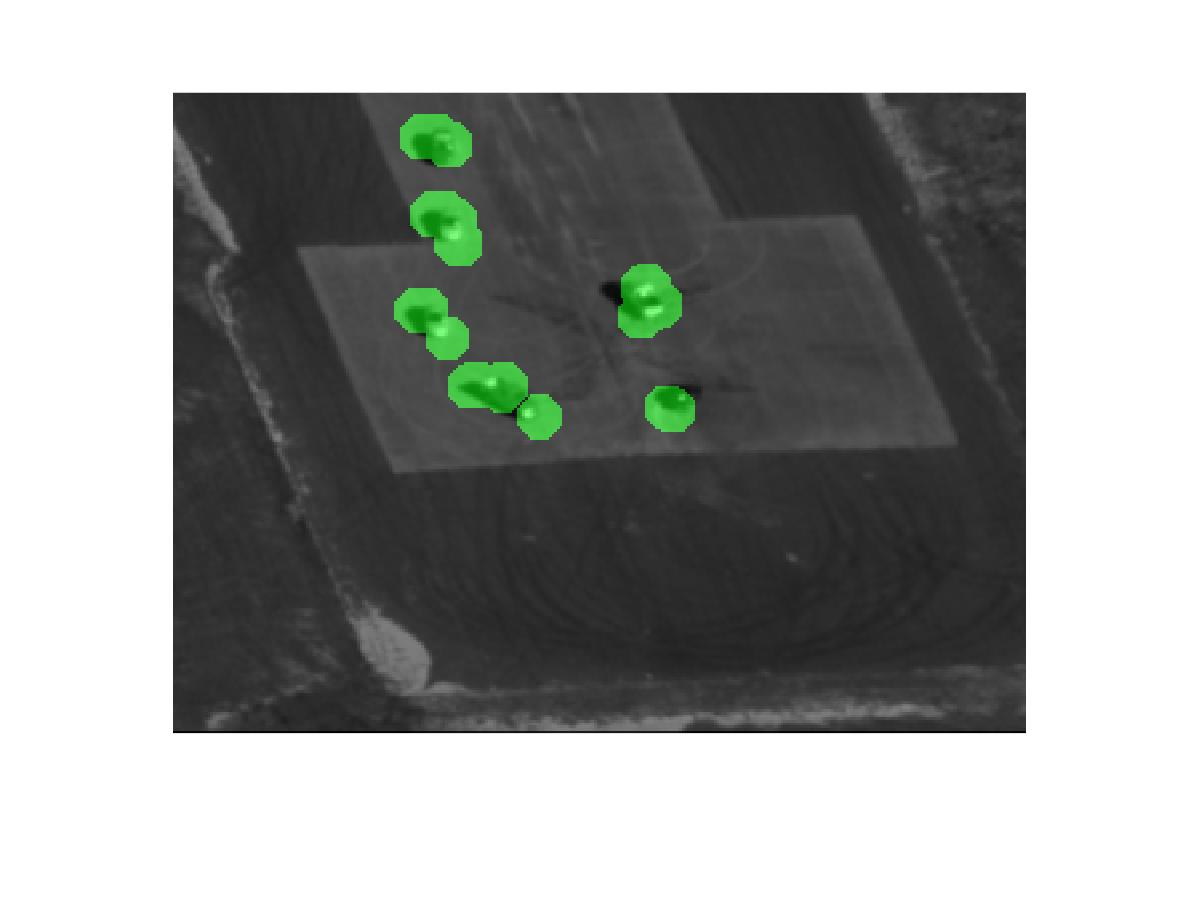
\includegraphics[trim=60mm 60mm 60mm 60mm,clip=true,width=0.23\linewidth]{../results/AerialFrame30.jpg} & 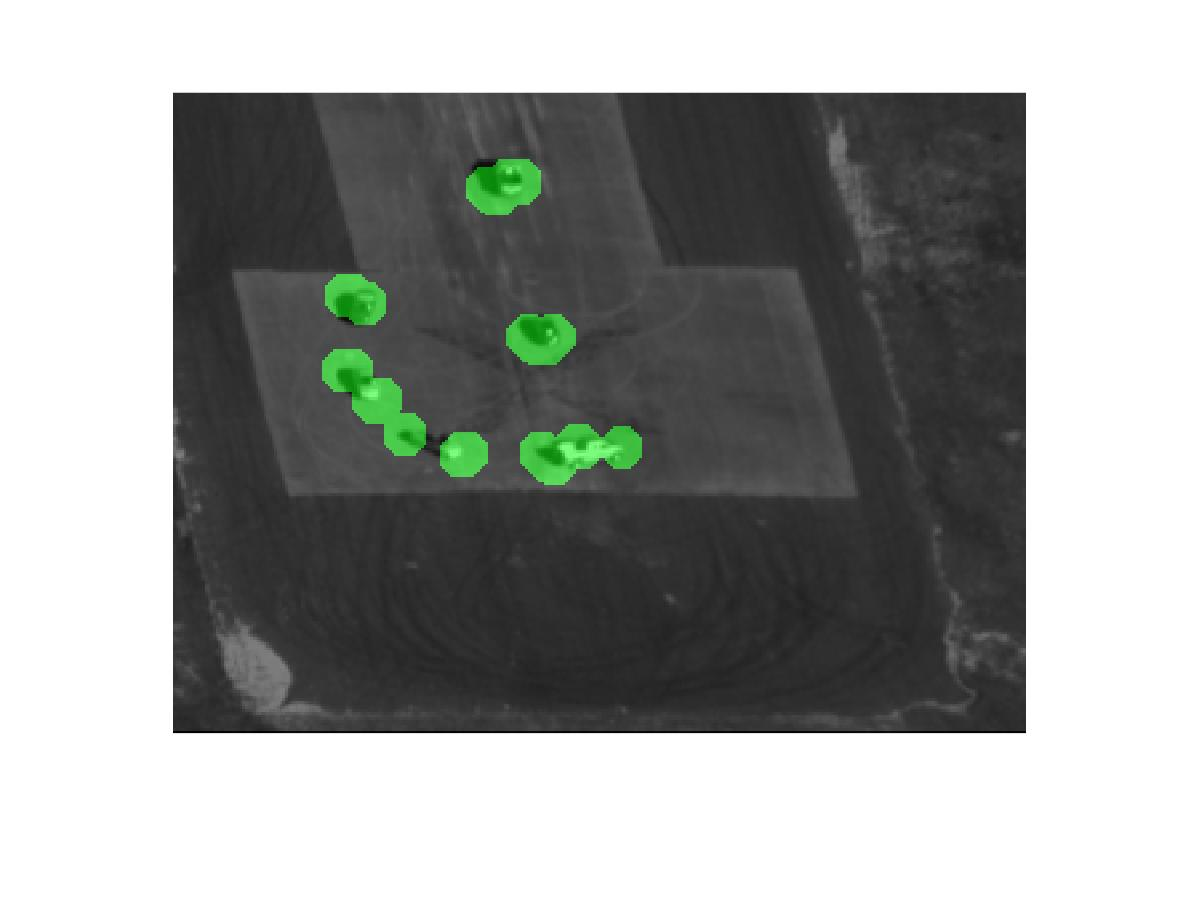
\includegraphics[trim=60mm 60mm 60mm 60mm,clip=true,width=0.23\linewidth]{../results/AerialFrame60.jpg} & 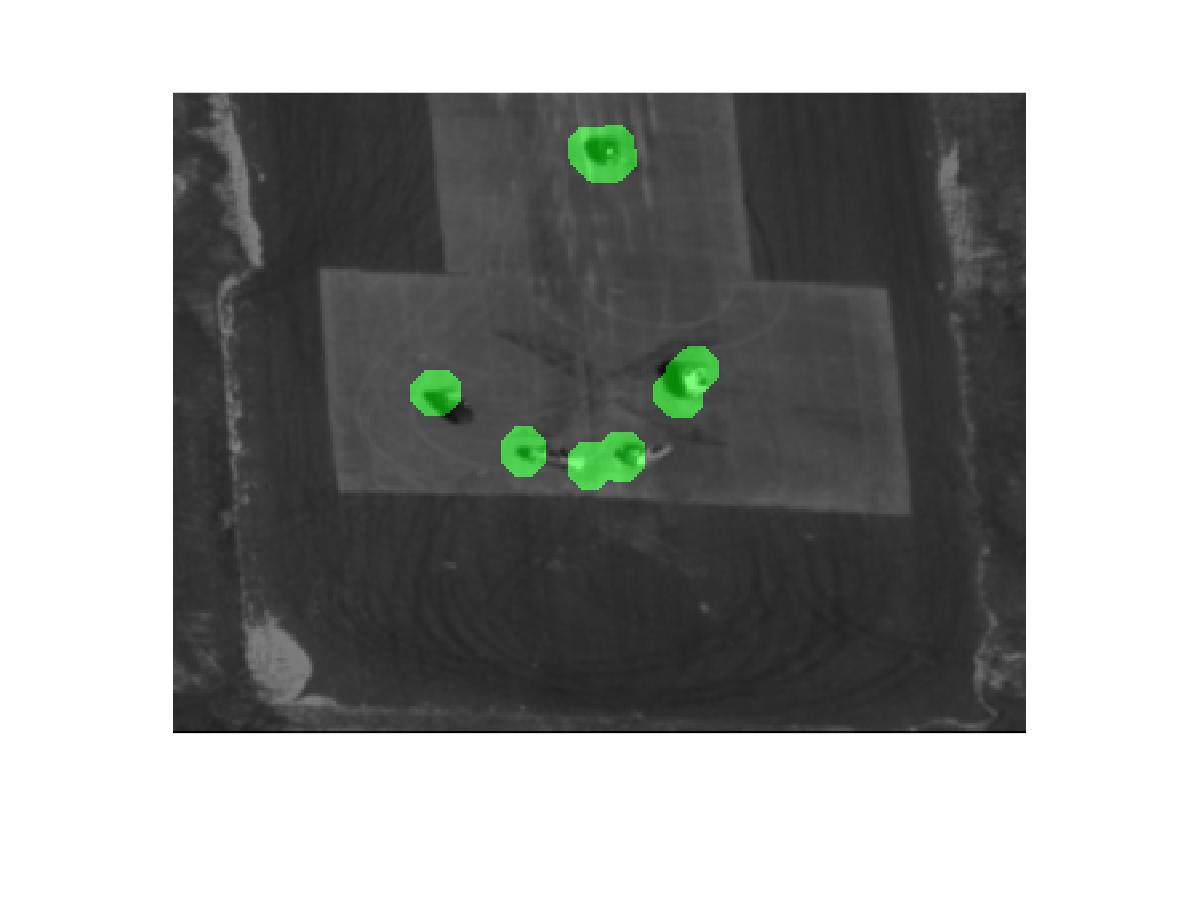
\includegraphics[trim=60mm 60mm 60mm 60mm,clip=true,width=0.23\linewidth]{../results/AerialFrame90.jpg} & 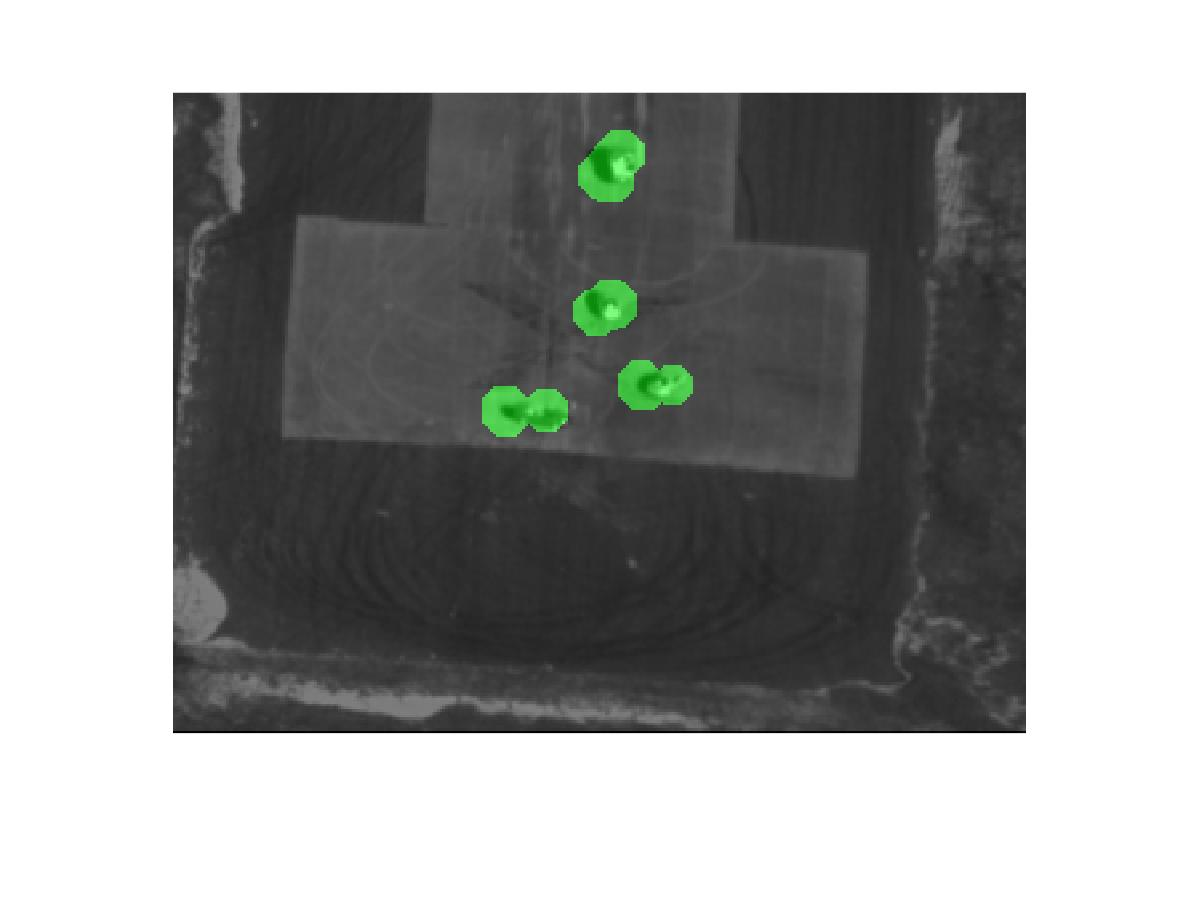
\includegraphics[trim=60mm 60mm 60mm 60mm,clip=true,width=0.23\linewidth]{../results/AerialFrame120.jpg} \\
\end{tabular}
\caption{Output of \texttt{testAerialSequence}}
\label{fig:testaerialsequence}
\end{figure*}

\end{document}

